\documentclass[a4paper]{article}
\usepackage[italian]{babel}
\usepackage[T1]{fontenc}
\usepackage[utf8]{inputenc}
\usepackage{soulutf8}
\usepackage{graphicx}
\usepackage{imakeidx}
\usepackage{enumitem}
\usepackage{amsfonts}
\usepackage{titlesec}
\usepackage{tabularx}
\usepackage{xcolor}
\usepackage{cancel}
\definecolor{mygrey}{HTML}{e6e6e6} %9fdfbf - c6ecd9
\definecolor{myblue}{RGB}{0, 80, 110}
\usepackage{tcolorbox}
\newtcolorbox{mybox}[1]{colback=gray!5!white,colframe=gray!75!black,fonttitle=\bfseries,title=#1}
\usepackage{soul} %for \hl
\sethlcolor{mygrey}
\newcommand{\sectionbreak}{\clearpage}
\makeindex[intoc]
\usepackage[hyperfootnotes=false, colorlinks=true, linkcolor=black, urlcolor=myblue]{hyperref}

\begin{document}
\title{Basi di Dati in Pillole}
\date{31 agosto 2019}
\author{\href{https://t.me/amarusofia}{Sofia Amarù}}
\maketitle
\tableofcontents

\section*{Note}
Il seguente testo è un personalissimo specchietto riassuntivo dei concetti fondamentali studiati durante il corso di Basi di Dati (corso di laurea triennale in Informatica presso l'Università degli Studi di Milano-Bicocca) e lo studio sullo stesso non è sufficiente per il superamento dell'esame. Si consiglia la lettura solo dopo aver studiato dal libro \emph{Basi di Dati - Modelli e linguaggi di interrogazione} degli autori Azteni, Ceri, Paraboschi, Torlone.\medskip\\
Questo testo può contenere errori: nell'eventualità vi prego di contattarmi per procedere alla correzione.\medskip\\
%
Ricordo ai miei compagni che l'esame è composto da 5 esericizi relativi ai seguenti argomenti:
\begin{itemize}[leftmargin=*, noitemsep]
  \item Modello ER
  \item Modello Relazionale
  \item Progettazione logica
  \item SQL
  \item Algebra relazionale
\end{itemize}

\section{Introduzione}
\subsection{Concetti fondamentali}
\subsubsection{Sistema informativo, sistema informatico, dati}

\hl{sistema informativo}: componente (non necessariamente automatizzata) di un’organizzazione, che gestisce le informazioni di interesse\medskip\\
%
\hl{sistema informatico}: porzione automatizzata del sistema informativo
\begin{itemize}[noitemsep]
  \item acquisizione e memorizzazione
  \item aggiornamento
  \item interrogazione
  \item elaborazione
\end{itemize}
%
\hl{dato $\neq$ informazione}
\begin{itemize}[noitemsep]
  \item dato: non ha alcun valore fino a quando non viene interpretato (immutato nel tempo)
  \item informazione: si ha quando un dato viene interpretato
\end{itemize}

\subsubsection{Definizione di database, DBMS}
\hl{DATABASE}: collezione di dati usati per rappresentare informazioni di interesse\\
\hl{DBMS (data base managment system)}: software per la gestione di DB

\subsubsection{Caratteristiche}
caratteristiche di un DB:
\begin{itemize}[noitemsep]
  \item privatezza
  \item affidabilità
  \item efficienza
  \item efficacia
\end{itemize}
%
fasi:
\begin{itemize}[noitemsep]
  \item definizione
  \item creazione e popolazione
  \item manipolazione
\end{itemize}
%
caratteristiche di un sistema di DB:
\begin{itemize}[noitemsep]
  \item natura autodescrittiva
  \item separazione tra programmi e dati
  \item astrazione dei dati (visione concettuale del DB per l'utente)
  \item supporto viste multiple dei dati
  \item condivisione dei dati e gestione con utenti multipli
\end{itemize}
%
\subsubsection{Modelli}
\hl{modello logico:}
\begin{itemize}[noitemsep]
  \item \hl{relazionale} (costruttore relazione; record a struttura fissa; tabella)
  \item gerarchico (strutture ad albero)
  \item reticolare (grafi)
  \item a oggetti
  \item XML
\end{itemize}
\hl{modello concettuale:}
\begin{itemize}[noitemsep]
  \item \hl{ER} (entità-relazione)
\end{itemize}

\subsubsection{Transizioni, schema, istanza}
transizione: insieme indivisibile di operazioni\medskip\\
%
\hl{schema}: struttura, invariante nel tempo\\
\hl{istanza}: valori attuali, possono cambiare anche molto rapidamente

\subsubsection{Livelli di astrazione}
\hl{schema logico} - descrizione dell’intera base di dati per mezzo del modello logico\\
\hl{schema interno} - rappresentazione dello schema logico per mezzo di strutture fisiche di memorizzazione\\
\hl{schema esterno} - descrizione di una porzione della base di dati per mezzo del modello logico. A volte non è esplicitamente presente ma è possibile definire relazioni derivate (viste)

\subsubsection{Indipendenza dei dati}
\hl{indipendenza fisica} - interagire col DBMS indipendentemente dalla struttura fisica dei dati\\
\hl{indipendenza logica} - interagire col livello esterno indipendentemente dal livello logico

\subsubsection{Linguaggi}
\hl{DDL Data Definition Language} - definizione degli schemi e delle autorizzazioni per l’accesso\\
\hl{DML Data Manipulation Language} - interrogazione e aggiornamento delle istanze del DB

\section{Modello ER (entità-relazione)}
\subsection{Rappresentazione grafica dei costrutti}
\begin{center}
      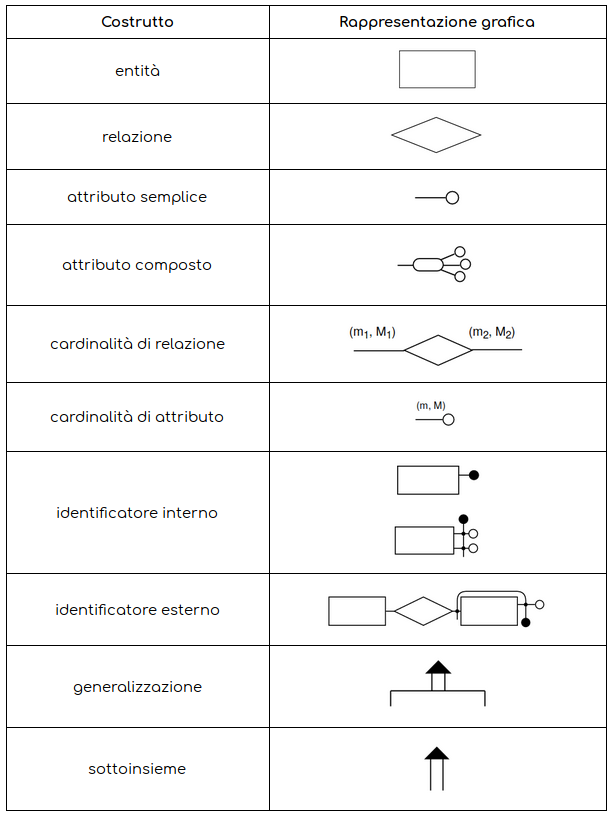
\includegraphics[scale=0.6]{img/er1.png}
\end{center}

\subsection{Costrutti}
\hl{entità} - classe di oggetti con proprietà comuni (il nome va al singolare)\medskip\\
\hl{relazione} - legame logico (il nome deve essere univoco; è preferibile usare un sostantivo per evitare di assegnare un verso)\medskip\\
\hl{attributo composto} - raggruppamento di attributi (Es. Via, Numero, CAP)\medskip\\
\hl{cardinalità} di relazione - indica quante volte, in una relazione, l'occorrenza dell'entità è legata ad occorrenze dell'altra entità
\begin{center}
      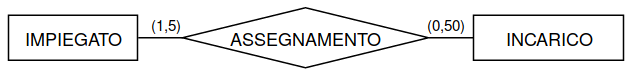
\includegraphics[scale=0.5]{img/er4.png}\\
      un impiegato ha da 1 a 5 incarichi
    \end{center}
\hl{identificatore (chiave)} - identificatore univoco dell’entità\medskip\\
\hl{identificatore interno} - se è uno o più attributi di un’entità
\begin{center}
      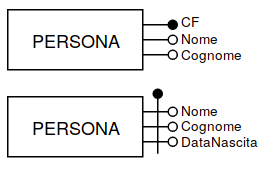
\includegraphics[scale=0.5]{img/er2.png}
\end{center}
\hl{identificatore esterno} - se un’entità viene identificata da un attributo di un’altra entità con cui ha una relazione
\begin{center}
      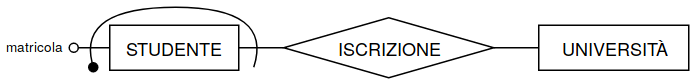
\includegraphics[scale=0.5]{img/er3.png}
\end{center}
\hl{generalizzazione totale} - non esistono altri figli
\begin{center}
      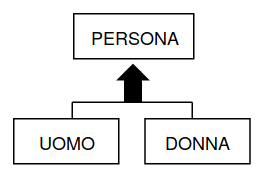
\includegraphics[scale=0.5]{img/er5.png}
\end{center}
\hl{generalizzazione parziale} - ci possono essere altri figli
\begin{center}
      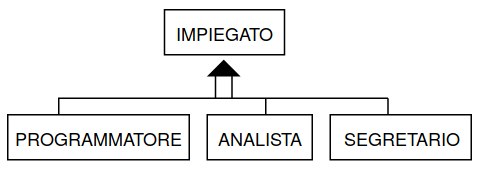
\includegraphics[scale=0.5]{img/er6.png}
\end{center}
\hl{sottoinsieme} - un solo figlio\medskip\\
\hl{generalizzazione esclusiva} - es. uomo-donna (o è uomo o è donna)\medskip\\
\hl{generalizzazione sovrapposta} - es. studente-lavoratore (può essere studente, lavoratore o studente-lavoratore)

\subsection{Esercizi}
\subsubsection{Esercizio 1}
Una grande città vuole rappresentare una parte del territorio in una base dati. Anzitutto vuole rappresentare le attuali linee metropolitane, ciascuna con un id (linea 1, linea 2, ecc.), un colore e una lunghezza in km. Ad ogni linea sono associate delle fermate, ciascuna identificata da un numero progressivo nell'ambito della linea (fermata 1 della linea 3, fermata 2 della linea 2, fermata 3 della linea 3 ecc.), da un nome (es. Castello, Duomo, ecc.) e da una profondità rispetto al piano strada. Quindi occorre assumere che una fermata di una linea, in cui transitano ovviamente treni nelle due direzioni, deve essere rappresentata come un'unica fermata.

Inoltre, si vuole rappresentare per ogni fermata quale sia la fermata successiva \underline{nella stessa linea}, e la distanza tra le due (es. la distanza tra le fermate 3 e 4 della linea 2 è di 700 metri).

Alcune coppie di fermate di due linee sono di incrocio tra due linee, in cui una linea passa <<sotto>> e l'altra passa <<sopra>>; si vuole rappresentare la relazione tra le due fermate (ad esempio, a piazzale Loreto della metro mlilanese si incrociano le linee rossa e verde. Questo significa che a Loreto corrispondono due distinte fermate, per esempio, la fermata 3 della linea rossa e la fermata 7 della linea verde, tra cui c'è una relazione di incrocio).
É facoltativo rappresentare i casi in cui vi siano incroci tra tre fermate.

Si vogliono poi rappresentare gli sponsor delle fermate (ad esempio l'azienda Prysmian è sponsor della fermata 2 della linea 7), con nome dello sponsor e sua partita iva. Ogni sponsor può esserlo di più fermate, ogni fermata può avere più sponsor. Gli sponsor pagano cifre mensili diverse per le diverse fermate, e anche questo attributo deve essere rappresentato nella base di dati.

Infine si vogliono rappresentare i principali edifici della città, con codice e nome delle'edificio. Gli edifici sono di due tipi: musei, di cui si vuole rappresentare il costo del biglietto, e monumenti, di cui si vuole rappresentare l'orario di apertura. Per i musei pubblici, e solo per quelli pubblici, si vuole rappresentare il giorno settimanale di accesso libero (lunedì, martedì, ecc.). Per ogni edificio si vuole rappresentare la fermata della metropolitana più vicina, con la distanza a piedi.\medskip\medskip\\
%
Rappresentare tutto mediante il modello ER, con identificatori, cardinalità minime e massime. Rappresentare lo schema ER in modo esteticamente gradevole.
\begin{center}
  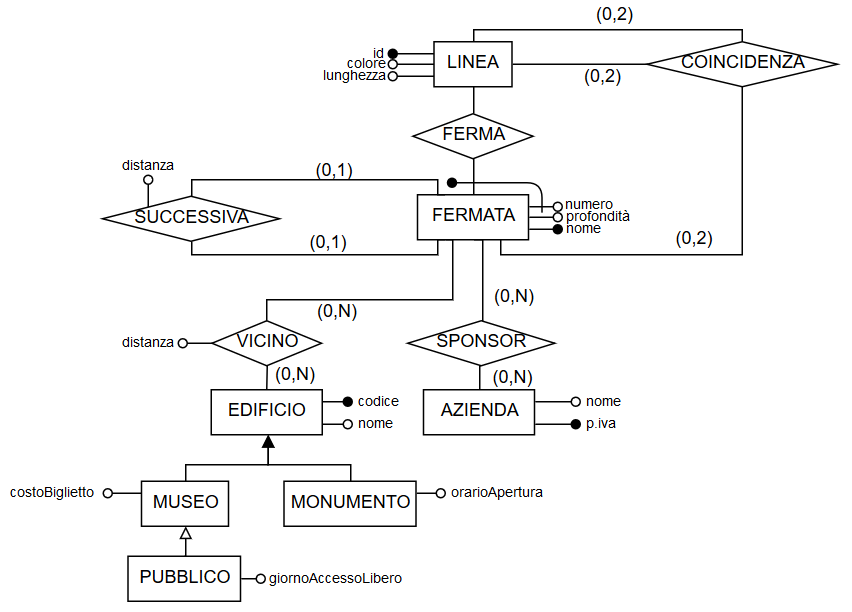
\includegraphics[scale=0.7]{img/es_er.png}
\end{center}

\subsubsection{Esercizio 2}
Il servizio di autoambulanze di una città deve organizzare un insieme di informazioni. Anzitutto ogni ambulanza è identificata da un codice, tipo automobile. Per ogni ambulanza si vuole poi rappresentare l'autorimessa di sosta, con via e numero civico, ed il personale assegnato, sempre lo stesso, con CF, nome, cognome, ruolo. Ogni chiamata è registrata con giorno, ora, minuto, persona chiamante, con CF, nome e cognome, e persona da trasportare, con CF, nome e cognome. Se la persona da trasportare è minorenne occorre rappresentare l'età. Deve poi essere rappresentato l'insieme dei ponti soccorso, con il nome, e che possono avere varie specializzazioni cioè generale, oftalmico, traumatologico, ecc. Quando l'ambulanza interviene deve essere associato alla chiamata (e quindi alla persona trasportata) una prima diagnosi, con codice, classificazione e nome, che permetta di capire quali ospedali possono offrire cure immediate; come conseguenza deve essere permanentemente rappresentata una relazione tra diagnosi e specializzazione
\begin{center}
      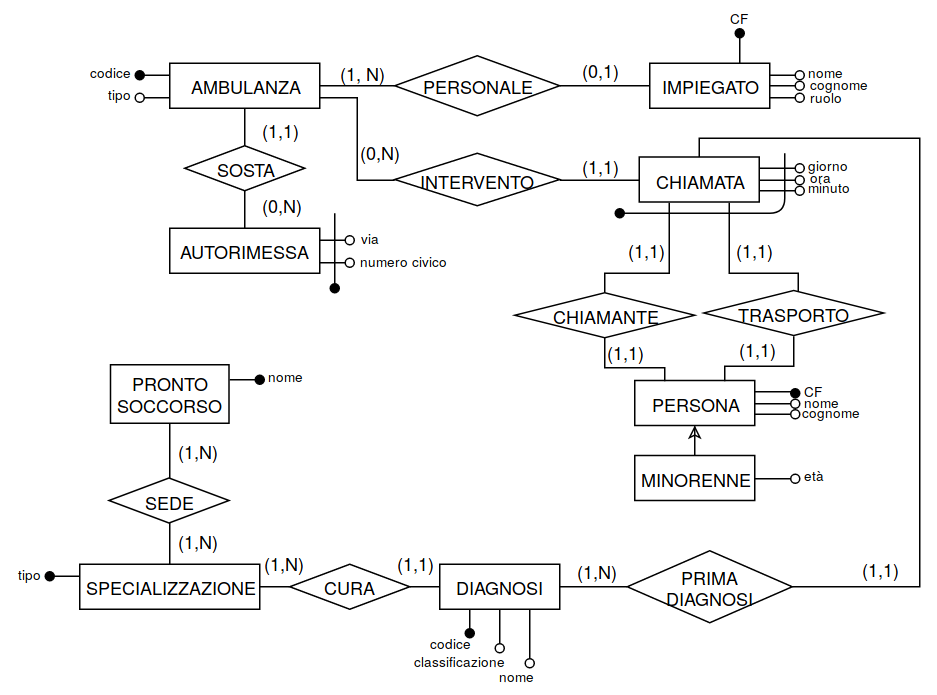
\includegraphics[scale=0.4]{img/er7.png}
\end{center}
\section{Modello Relazionale}
\subsection{Vincoli di integrità}
\hl{intrarelazionale} - soddisfatto rispetto a singole relazioni
\begin{itemize}
  \item[] \hl{di tupla} -  può essere valutato su ciascuna tupla indipendentemente dalle altre.\\
  Es. la lode può comparire solo con voto 30
  \item[] \hl{di dominio} - restrizione sul dominio dell’attributo\\
  Es. voto compreso tra 18 e 30
\end{itemize}
\hl{interrelazionale} - coinvolge più relazioni
\begin{itemize}
  \item[] \hl{vincolo di integrità referenziale} - proprietà dei dati che per essere soddisfatta richiede che ogni valore di un attributo (colonna) di una relazione (tabella) esista come valore di un altro attributo in un'altra relazione.\\
  Es. matricola compare in ESAMI solo se compare in STUDENTI
\end{itemize}

\subsection{Chiave, superchiave, superchiave minimale}
\hl{chiave} - insieme di attributi utilizzato per identificare univocamente le tuple di una relazione\medskip\\
\hl{superchiave} - insieme di attributi di una relazione tali che le relative tuple sono tutte diverse tra loro (identificazione univoca)\medskip\\
\hl{superchiave minimale} - superchiave che non contiene una superchiave\medskip\\
\hl{chiave primaria} - chiave a cui non è permesso contenere valori nulli (la presenza di NULL impedisce l’identificazione univoca)

\subsection{Esercizi}
\subsubsection{Esercizio 1}
La seguente base di dati rappresenta l’archivio di una banca. La banca ha diverse filiali. I conti correnti possono avere un intestatario ed eventualmente un cointestatario. Alcuni clienti hanno più di un conto. Si tiene traccia anche di eventuali conti chiusi. I movimenti sui conti possono essere effettuanti in filiale da un operatore, oppure via WEB, in questo caso non risulta alcun operatore associato a quel movimento. I clienti possono stipulare al massimo un mutuo in un dato giorno, ed effettuare al massimo un movimento in una data ora di un giorno.\medskip\medskip\\
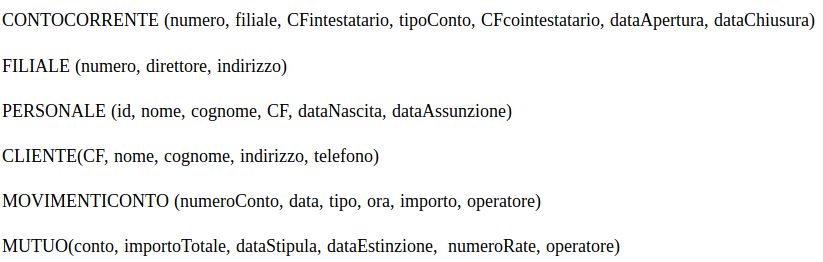
\includegraphics[scale=0.4]{img/rel1.png}
%
Definire tutte le chiavi primarie e i tutti i vincoli di integrità referenziale. Le chiavi primarie ed i vincoli di integrità referenziale possono essere espressi in modo grafico direttamente sul testo. I vincoli di integrità referenziale possono essere espressi in  modo grafico.\medskip\\
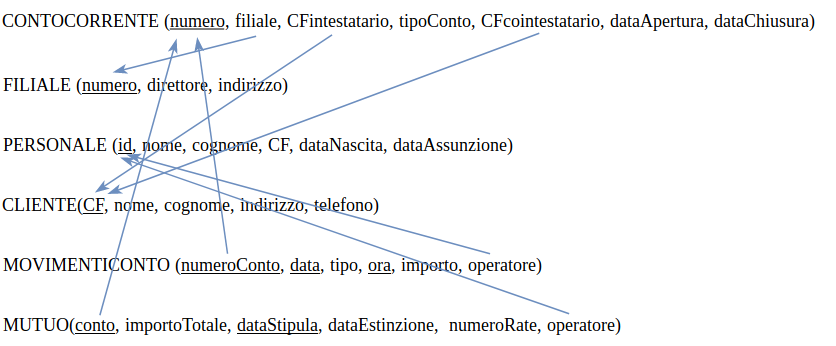
\includegraphics[scale=0.4]{img/rel2.png}\medskip\medskip\\
Indicare:
\begin{enumerate}[leftmargin=*]
  \item un vincolo di dominio \\importo > 0 in MOVIMENTICONTO
  \item un vincolo di ennupla \\dataApertura antecedente dataChiusura in CONTOCORRENTE
  \item una superchiave non minimale \\CF, nome, cognome in CLIENTE
  \item una chiave che non sia stata scelta come chiave primaria \\CF in PERSONALE
  \item due attributi che possano assumere valore NULL \\operatore in MOVIMENTICONTO;\\dataChiusura in CONTOCORRENTE
\end{enumerate}


\section{Progettazione logica}
\subsection*{Fasi}
\begin{itemize}[noitemsep, leftmargin=*]
  \item \hl{Ristrutturazione schema ER}
        \begin{itemize}[noitemsep]
          \item Analisi delle ridondanze
          \item Eliminazione delle generalizzazioni
          \item Partizionamento/accorpamento entità e associazioni
          \item Scelta identificatori principali
        \end{itemize}
  \item \hl{Traduzione verso modello logico}
\end{itemize}

\subsection{Ristrutturazione schema ER}
\subsubsection{Analisi delle ridondanze}
La presenza di un dato ridondante comporta:
\begin{itemize}[noitemsep]
  \item[$\times$] occupazione memeoria
  \item[$\times$] operazioni per mantenere dato aggiornato
  \item[\checkmark] riduzione accessi necessari per calcolarlo
\end{itemize}

\subsubsection{Eliminazione delle generalizzazioni}
\hl{Accorpamento dei figli nel genitore}
Si usa quando l'accesso alle entità è contestuale.
\begin{center}
      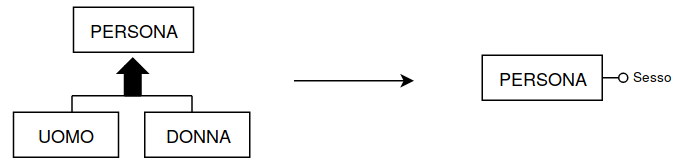
\includegraphics[scale=0.45]{img/pl1.png}
\end{center}
%
\hl{Accorpamento del genitore dei figli}\\
NB. Possibile solo se la generalizzazione è totale!
\begin{center}
      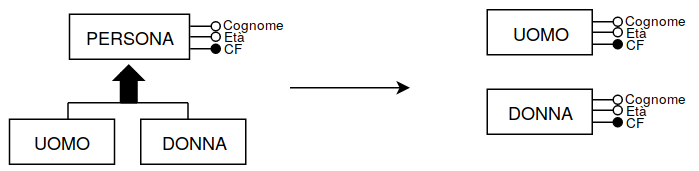
\includegraphics[scale=0.45]{img/pl2.png}
\end{center}
%
\hl{Sosituzione generalizzazioni con associazioni} Si usa quando l'accesso alle due entità è separato.
\\NB. Conveniente con generalizzazione parziale
\begin{center}
      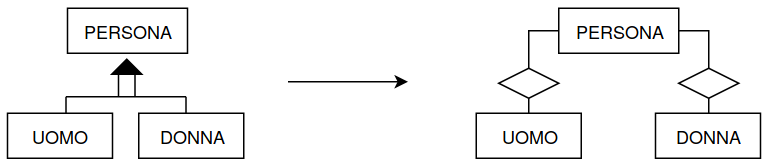
\includegraphics[scale=0.45]{img/pl3.png}
\end{center}

\subsubsection{Partizionamento}
\hl{decomposizione verticale}
\begin{center}
      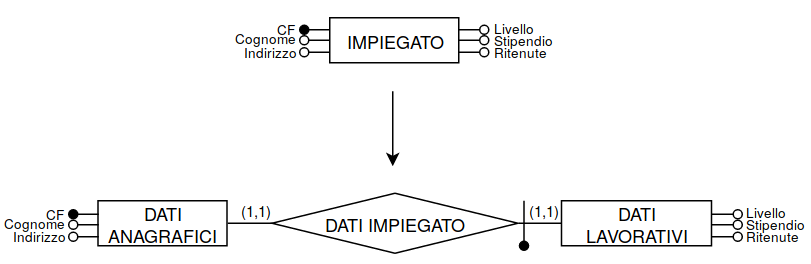
\includegraphics[scale=0.45]{img/pl4.png}
\end{center}
%
\hl{decomposizione orizzontale}
\begin{center}
      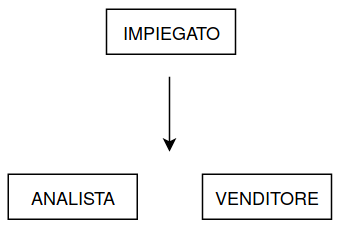
\includegraphics[scale=0.45]{img/pl5.png}
\end{center}

\subsubsection{Eliminazione di attributi multivalore}
Es. Un'agenzia può avere più numeri di telefono
\begin{center}
      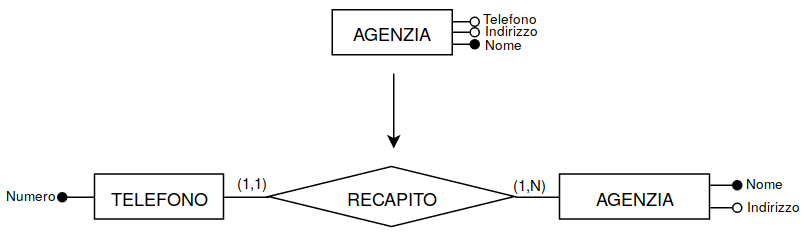
\includegraphics[scale=0.44]{img/pl6.png}
\end{center}

\subsubsection{Accorpamento di entità}
NB. Solitamente su associazioni uno a uno
\begin{center}
      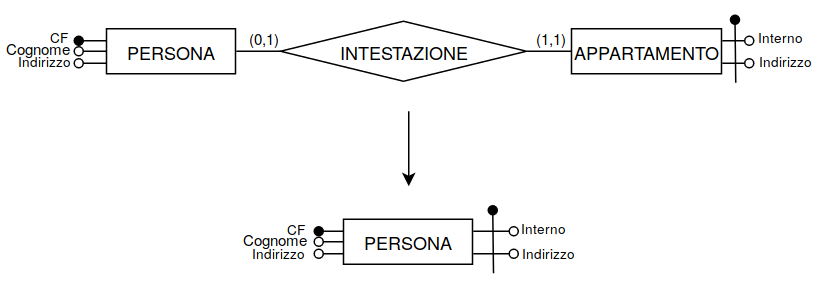
\includegraphics[scale=0.44]{img/pl7.png}
\end{center}

\subsubsection{Scelta degli identificatori principali}
\begin{itemize}[noitemsep]
  \item No attributi con valori nulli
  \item Preferire identificatore composto da 1 o \textbf{pochi} attributi
  \item Preferire identificatore interno ad intentificatore esterno
  \item Preferire identificatore che viene utilizzato da molte operazioni per accedere alle occorrenze dell'entità
\end{itemize}

\subsection{Traduzione verso modello logico}
\subsubsection{Molti a molti}
\begin{center}
      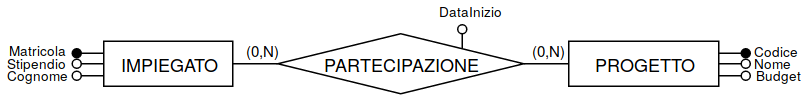
\includegraphics[scale=0.44]{img/pl8.png}
\end{center}
%
IMPIEGATO(\underline{Matricola}, Cognome, Stipendio)\\
PROGETTO(\underline{Codice}, Nome, Budget)\\
PARTECIPAZIONE(\underline{Impiegato}, \underline{Progetto}, DataInizio)\medskip\\
%
\hl{NB.} \underline{Impiegato} è la ridenominazione di \underline{Matricola} e \underline{Progetto} è la ridenominazione di \underline{Codice}

\subsubsection{Uno a molti}
\begin{center}
      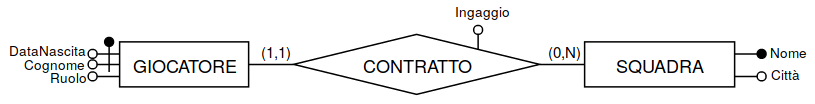
\includegraphics[scale=0.44]{img/pl9.png}
\end{center}
%
GIOCATORE(\underline{DataNascita}, \underline{Cognome}, Ruolo)\\
SQUADRA(\underline{Nome}, Città)\\
CONTRATTO(\underline{Giocatore}, Squadra, Ingaggio)\medskip\\
%
diventa\medskip\\
%
GIOCATORE(\underline{DataNascita}, \underline{Cognome}, Ruolo, Squadra, Ingaggio)\\
SQUADRA(\underline{Nome}, Città)

\subsubsection{Uno a uno con partecipazioni obbligatorie per entrambe le entità}
\begin{center}
      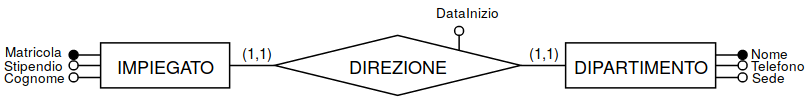
\includegraphics[scale=0.44]{img/pl10.png}
\end{center}
%
DIRETTORE(\underline{Matricola}, Cognome, Stipendio, Dipartimento, InizioDirezione)\\
DIPARTIMENTO(\underline{Nome}, Telefono, Sede)\medskip\\
%
oppure\medskip\\
%
DIRETTORE(\underline{Matricola}, Cognome, Stipendio)\\
DIPARTIMENTO(\underline{Nome}, Telefono, Sede, Direttore, InizioDirezione)

\subsubsection{Uno a uno con partecipazione opzionale per una sola entità}
\begin{center}
      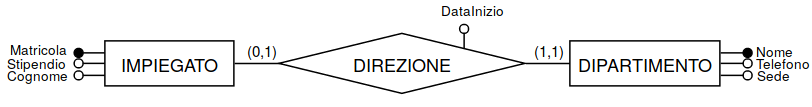
\includegraphics[scale=0.44]{img/pl11.png}
\end{center}
%
IMPIEGATO(\underline{Matricola}, Cognome, Stipendio)\\
DIPARTIMENTO(\underline{Nome}, Telefono, Sede)\\
DIREZIONE(\underline{Direttore}, Dipartimento, DataInizio)

\subsubsection{Attributi opzionali}
Gli attributi opzionali vengono contrassegnati con il simbolo *
\begin{center}
      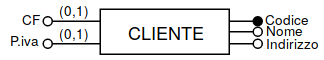
\includegraphics[scale=0.5]{img/pl12.png}
\end{center}
%
CLIENTE(\underline{Codice}, Nome, Indirizzo, CF*, P.iva*)

\subsection{Esercizi}
\subsubsection{Esercizio 1}
Dato il seguente schema Entità-Relazione, produrre lo schema ristrutturato e semplificato, tenendo presente che la grande maggioranza delle operazioni opera separatamente sulle entità E5 ed E4.
\begin{center}
      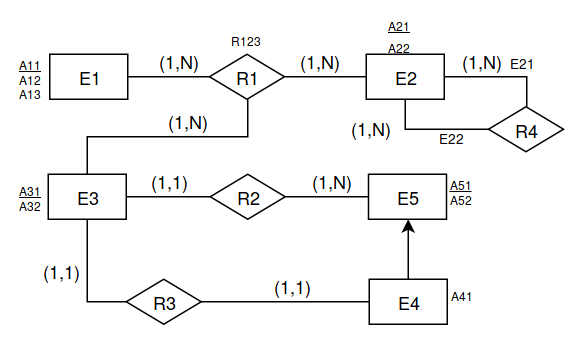
\includegraphics[scale=0.5]{img/pl13.png}
\end{center}
Soluzione:
\begin{center}
      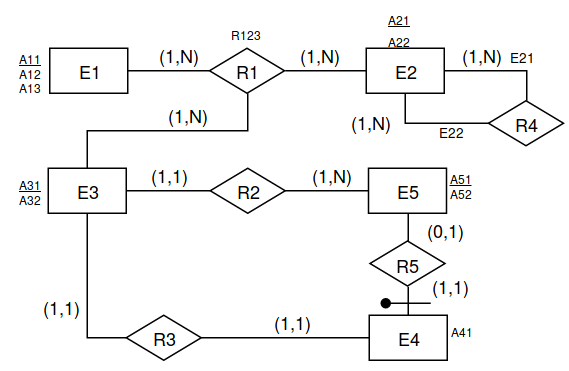
\includegraphics[scale=0.5]{img/pl14.png}
\end{center}
E1(\underline{A11}, A12, A13)\\
E2(\underline{A21}, A22)\\
R1(\underline{A11}, \underline{A21}, \underline{A31})\\
R4(\underline{A21-1}, \underline{A21-2})\\
E3(\underline{A31}, A32, A51-1, A51-2)\\
\cancel{R2()}\\
E5(\underline{A51}, A52)\\
\cancel{R3()}\\
E4(\underline{A51}, A41)\\
\cancel{R5()}
\section{Algebra relazionale}
\hl{Relazione}: insieme di tuple omogenee.

\subsection{Operatori insiemistici}
\hl{unione} $\cup$ \\
\hl{intersezione} $\cap$\\
\hl{differenza} $-$
\begin{center}
      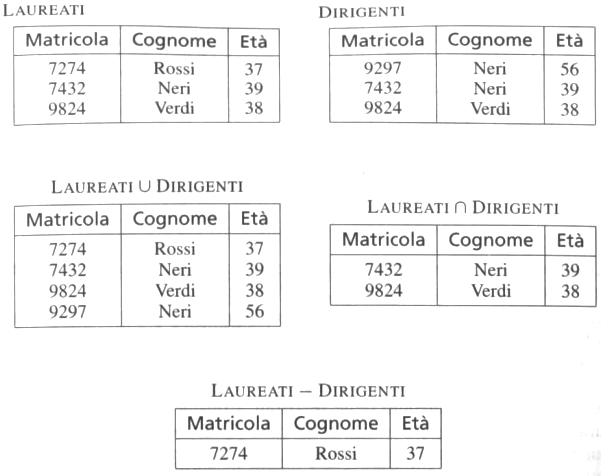
\includegraphics[scale=0.45]{img/ar1.png}
\end{center}

\subsection{Operatori principali}
\subsubsection{Ridenominazione}
Agisce solo sullo schema, cambiando solo i nomi degli attributi
\[\rho_{\textbf{nuovo nome}\leftarrow \textbf{vecchio nome}}\]
\begin{center}
      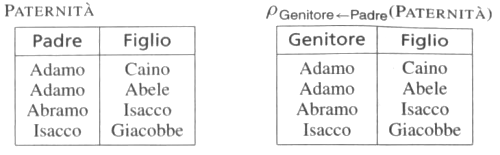
\includegraphics[scale=0.45]{img/ar2.png}
\end{center}

\subsubsection{Selezione}
Produce un sottoinsieme delle tuple su tutti gli attributi (decomposizione orizzontale)
\[\sigma_{\textbf{condizione di selezione}}\]
\begin{center}
      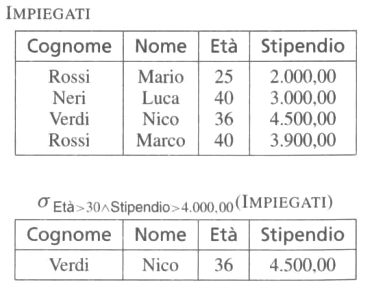
\includegraphics[scale=0.45]{img/ar3.png}
\end{center}

\subsubsection{Proiezione}
È l’insieme delle tuple ottenute considerando solo i valori dei campi scelti. La proiezione contiene lo stesso numero di tuple della relazione di partenza solo se i campi scelti sono una superchiave. (decomposizione verticale)
\[\pi_{\textbf{campi scelti}}\]
\begin{center}
      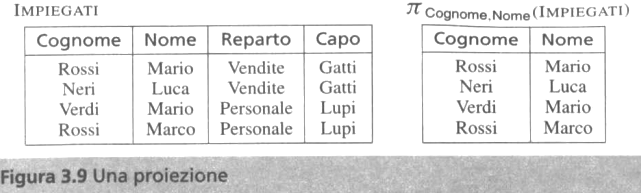
\includegraphics[scale=0.45]{img/ar4.png}\\
      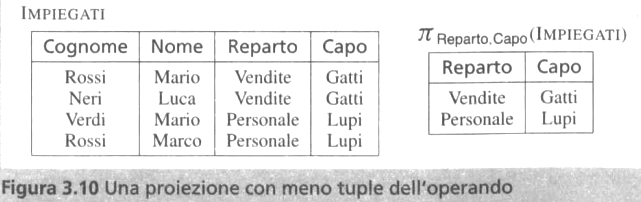
\includegraphics[scale=0.45]{img/ar5.png}
\end{center}

\subsubsection{Join}
Permette di correlare dati contenuti in relazioni diverse
\[\Join_{\textbf{uguaglianza tra campi}}\]
%
\hl{join naturale} - correla dati in relazioni diverse sulla base di valori uguali in campi uguali.
\begin{center}
      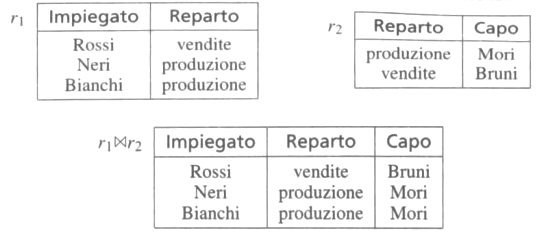
\includegraphics[scale=0.45]{img/ar6.png}
\end{center}
%
\hl{join completo} - ogni tupla contribuisce ad almeno una tupla del risultato (vedi immagine sopra)\medskip\\
%
\hl{join con tuple dangling} - alcune tuple non contribuiscono al risultato
\begin{center}
      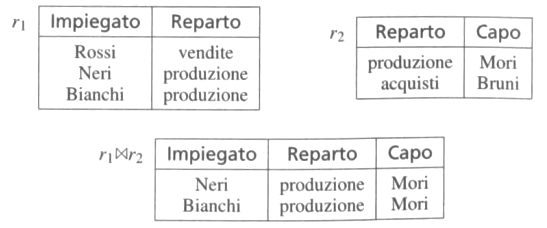
\includegraphics[scale=0.45]{img/ar7.png}
\end{center}
%
\hl{join esterni} - tutte le tuple contribuiscono al risultato, eventualmente estese con valori nulli
\begin{itemize}[noitemsep]
  \item [-] sinistro
  \item [-] destro
  \item [-] completo
\end{itemize}
\begin{center}
      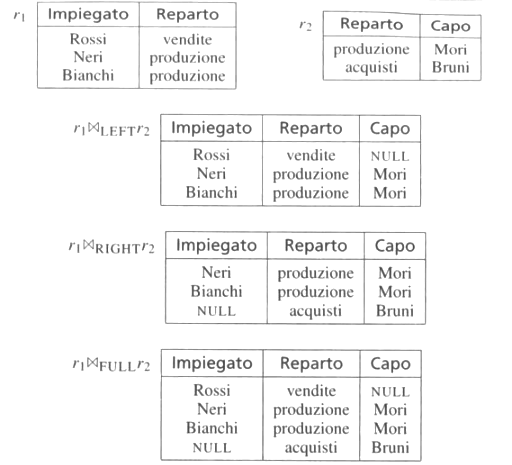
\includegraphics[scale=0.45]{img/ar8.png}
\end{center}

\subsubsection{Prodotto cartesiano}
Il risultato è la combinazione delle tuple in tutti i modi possibili.\\
\hl{NB}. il termine è improprio: il prodotto cartesiano di due insiemi è un insieme di coppie, qui abbiamo tuple.
\begin{center}
      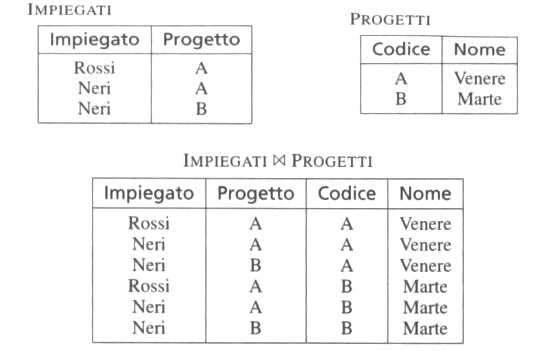
\includegraphics[scale=0.45]{img/ar9.png}
\end{center}

\subsubsection{Theta join e equi-join}
\hl{theta join} - operatore derivato, prodotto cartesiano + selezione\medskip\\
\hl{equi-join} - theta join in cui la condizione di selezione è una congiunzione di atomi di uguaglianza con un attributo della prima relazione
\begin{center}
      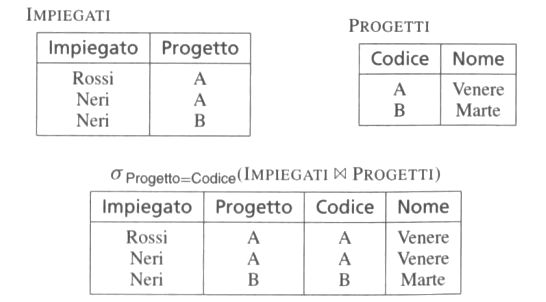
\includegraphics[scale=0.45]{img/ar10.png}
\end{center}

\subsubsection{Logica a tre valori}
vero (V), falso (F), sconosciuto (U)
\begin{center}
      
\includegraphics[scale=0.45]{img/ar11.png}
\end{center}

\subsubsection{Interrogazioni}
\hl{Interrogazione}: funzione che, applicata alla base di dati, produce relazioni.

\subsection{Esercizi}
\subsubsection{Esercizio 1}
Date le relazioni\medskip\\
STUDENTE(\underline{mat}, nome, cognome, cittàNascita)\\
ESAME(\underline{matricola}, \underline{codiceCorso}, voto, data)\\
CORSO(\underline{codiceCorso}, nomeCorso, docente, annoCreazione)

\begin{enumerate}
  \item Trovare nome, cognome e matricola degli studenti che hanno superato l'esame di almeno un corso successivo alla data 10/10/2015
  \item Trovare nome, cognome e matricola degli studenti che non hanno superato alcun esame (nota: solo gli esami con voto positivo vengono registrati nella relazione esame) dopo la data 10/10/2015
  \item Trovare nome, cognome e matricola degli studenti omonimi (stesso nome e cognome) che sono nati nella stessa città
\end{enumerate}

\begin{mybox}{}
  Abbiamo le seguenti tabelle:\medskip\\
  \begin{tabular}{|c|c|c|c|}
    \hline
    \multicolumn{4}{|c|}{STUDENTE}\\
    \hline
    \underline{mat} & nome & cognome & cittàNascita\\
    \hline
  \end{tabular}
\medskip

\begin{tabular}{|c|c|c|c|}
  \hline
  \multicolumn{4}{|c|}{ESAME}\\
  \hline
  \underline{matricola} & \underline{codiceCorso} & voto & data\\
  \hline
\end{tabular}
\medskip

\begin{tabular}{|c|c|c|c|}
  \hline
  \multicolumn{4}{|c|}{CORSO}\\
  \hline
  \underline{codiceCorso} & nomeCorso & docente & annoCreazione\\
  \hline
\end{tabular}
\medskip\medskip\\
%
Ricordiamo come opera il join:\medskip\\
\begin{tabular}{|c|c|c|c|c|c|c|}
  \hline
  \multicolumn{7}{|c|}{STUDENTE $\Join_{mat=matricola}$ ESAME}\\
  \hline
  mat & nome & cognome & cittàNascita & codiceCorso & voto & data\\
  \hline
\end{tabular}
\medskip

\begin{tabular}{|c|c|c|c|c|c|c|}
  \hline
  \multicolumn{7}{|c|}{ESAME $\Join$ CORSO}\\
  \hline
  matricola & codiceC. & voto & data & nomeC. & docente & annoC.\\
  \hline
\end{tabular}
\medskip\\
%
Soluzioni:
\begin{enumerate}
  \item $\pi_{nome, cognome, mat}$($\sigma_{annoCreazione>2015}$((STUDENTE $\Join_{mat=matricola}$ ESAME) $\Join$ CORSO))
  \item $\pi_{nome, cognome, matricola}$(STUDENTE)-($\pi_{nome, cognome, matricola}$ ($\sigma_{data>10/10/2015}$(STUDENTE $\Join_{mat=matricola}$ ESAME)))
  \item $\pi_{nome, cognome, matricola}$($\rho_{nome1, cognome1, citta1}$ $\leftarrow _{nome, cognome, cittaNascita}$(STUDENTE) $\Join_{nome1=nome \land cognome1=cognome \land citta1=cittaNascita}$ STUDENTE)
\end{enumerate}
\end{mybox}

\subsubsection{Esercizio 2}
Date le relazioni:\medskip\\
STUDENTE(\underline{mat}, nome, cognome)\\
ESAME(\underline{mat}, \underline{codCorso}, voto, data)\\
CORSO(\underline{codCorso}, nomeCorso, docnte)

\begin{enumerate}
  \item Trovare nome, cognome e matricola degli studenti che hanno superato l'esame di almeno un corso
  \item Trovare nome, cognome e matricola degli studenti che non hanno superato alcun esame (nota: solo gli esami con voto positivo vengono registrati nella relazione esame)
  \item Trovare la matricola degli studenti che abbiano superato sia basi di dati che analisi (entrambi gli esami)
\end{enumerate}

\begin{mybox}{}
\begin{enumerate}
  \item $\pi_{nome, cognome, mat}$(STUDENTE $\Join$ ESAME)
  \item $\pi_{nome, cognome, mat}$(STUDENTE)$- \pi_{nome, cognome, mat}$(STUDENTE $\Join$ ESAME)
  \item $\pi_{nome, cognome, mat}$(($\sigma_{corso.nomeCorso='Basi\ di\ dati'}$(STUDENTE $\Join$ ESAME $\Join$ CORSO)) $\land$ ($\sigma_{corso.nomeCorso='Analisi'}$(STUDENTE $\Join$ ESAME $\Join$ CORSO)))
\end{enumerate}
\end{mybox}

\subsubsection{Esercizio 3}
Si consideri il seguente schema  relativo a una base di dati che raccoglie i turni degli assistenti di volo di una compagnia aerea. Il grado dell'assistente di volo può essere 'junior' o 'senior'. Per il turno, si suppone che un assistente di volo possa fare una sola tratta andata e ritorno al giorno (per esempio, nella stessa giornata può effettuare solo due viaggi sulla tratta Milano-Roma).\medskip\\
AssistenteDiVolo(\underline{CodiceA}, Nome, Cognome, Genere, Grado, DataNascita)\\
Volo(\underline{CodiceVolo}, Provenienza, Destinazione)\\
Turno(\underline{CodiceVolo}, \underline{CodiceA}, \underline{Data})

\begin{enumerate}
  \item Trovare nome, cognome e data di nascita degli assistenti di volo di genere femminile con grado senior che abbiano effettuato il 22 giugno 2007 un volo Milano-Roma e un volo Roma-Atene.
\end{enumerate}

\begin{mybox}{}
$\pi_{nome, cognome, dataNascita}$($\sigma_{genere='F' \land grado='senior' \land data='22/06/2007'}$ (ASSISTENTE $\Join$ TURNO $\Join$ ($\sigma_{provenienza='Milano' \land destinazione='Roma'}$ (VOLO) $\cup$ $\sigma_{provenienza='Roma' \land destinazione='Atene'}$(VOLO))))
\end{mybox}


\section{SQL}
L'SQL (\emph{Structured Query Language}) è un linguaggio standardizzato per database basati sul modello relazionale (RDBMS), progettato per le seguenti operazioni:
\begin{itemize}
  \item creare e modificare schemi di database (\textbf{DDL} = Data Definition Language);
  \item inserire, modificare e gestire dati memorizzati (\textbf{DML} = Data Manipulation Language);
  \item interrogare i dati memorizzati (\textbf{DQL}= Data Query Language);
  \item creare e gestire strumenti di controllo e accesso ai dati (\textbf{DCL} = Data Control Language).
\end{itemize}
%
É dunque un linguaggio per interrogare e gestire basi di dati mediante l'utilizzo di costrutti di programmazione denominati \textbf{query}. La maggior parte delle implementazioni dispongono di interfaccia alla riga di comando per l'esecuzione diretta di comandi, in alternativa alla sola interfaccia grafica GUI.

\subsection{Operatori}
Gli operatori messi a disposizione dall'SQL standard si dividono in sette categorie:
\begin{itemize}[noitemsep]
  \item Operatori di assegnazione
  \item Operatori di confronto
  \item Operatori stringa
  \item Operatori aritmetici
  \item Operatori condizionali
  \item Operatori logici
  \item Operatori tra bit
\end{itemize}

\subsubsection{Operatori di assegnazione}
\begin{tabularx}{350pt}{|l|X|}
  \hline
  = & Esprime un'assegnazione e non restituisce alcun valore.\\
  \hline
  := & Esprime un'assegnazione di un valore ad una variabile non ancora istanziata e non restituisce alcun valore.\\
  \hline
\end{tabularx}

\subsubsection{Operatori di confronto}
\begin{tabularx}{350pt}{|l|X|}
  \hline
  = &  Esprime uguaglianza tra due valori numerici o stringhe di caratteri (dove non è usato come operatore di assegnazione)\\
  \hline
  IS & Si usa per verificare se un valore è NULL, oppure se corrisponde a un valore booleano (TRUE, FALSE, UNKNOWN).\\
  \hline
  LIKE & Esprime somiglianza tra due valori letterali. É possibile usare, per i confronti, i caratteri speciali \% (sostituisce un arbitrario numero di lettere) e \_ (sostituisce una lettera arbitraria)\\
  \hline
  < & Minore\\
  \hline
  > & Maggiore\\
  \hline
  <= & Minore o uguale\\
  \hline
  >= & Maggiore o uguale\\
  \hline
  <> & Diverso\\
  \hline
  != & Diverso\\
  \hline
  BETWEEN ... AND & Recupera un valore compreso tra due valori\\
  \hline
  IN & Stabilisce se un valore è contenuto in una lista di valori possibili\\
  \hline
  EXISTS & Stabilisce se una determinata subquery restituisce un valore\\
  \hline
  ANY o SOME & Stabilisce se una determinata subquery restituisce almeno uno dei valori specificati\\
  \hline
  ALL & Stabilisce se una determinata subquery restituisce tutti i valori desiderati\\
  \hline
\end{tabularx}

\paragraph{Operatori contrari} \ \medskip\\
\begin{tabular}{|l|}
  \hline
  IS NOT\\
  \hline
  NOT LIKE\\
  \hline
  NOT BETWEEN\\
  \hline
  NOT IN\\
  \hline
  NOT EXISTS\\
  \hline
\end{tabular}

\subsubsection{Operatori aritmetici}
\begin{tabularx}{350pt}{|l|X|}
  \hline
  + & Addizione\\
  \hline
  - & Sottrazione\\
  \hline
  * & Moltiplicazione\\
  \hline
  / & Divisione\\
  \hline
  MOD & Restituisce il resto di una divisione\\
  \hline
  DIV & Restituisce la parte intera di una divisione\\
  \hline
\end{tabularx}

\subsubsection{Operatori condizionali}
L'unico operatore condizionale di SQL è WHERE (\emph{dove}, vedi 6.2.1) e serve a definire criteri di ricerca mirati.

\subsubsection{Operatori logici}
\begin{tabularx}{350pt}{|l|X|}
  \hline
  AND & Restituisce il valore TRUE se e solo se entrambi gli operandi sono veri.\\
  \hline
  OR & Restituisce TRUE se e solo se almeno uno degli operandi è vero.\\
  \hline
  NOT & Restituisce falso se questo è vero, vero se questo è falso.\\
  \hline
  XOR & Restituisce TRUE se e solo se uno solo degli operandi è vero.\\
  \hline
\end{tabularx}

\subsection{Interrogazioni}
\begin{center}
      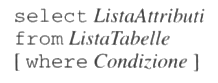
\includegraphics[scale=0.5]{img/sql1.png}\\
      esempio di interrogazione
\end{center}

\subsubsection{Select, from, where}
clausola \hl{\texttt{select}} (target list) - specifica gli elementi dello schema della tabella risultato. Come argomento può comparire * , che rappresenta tutti gli attributi delle tabelle elencate nella clausola from.\medskip\\
%
clausola \hl{\texttt{from}} - ha come argomento l’insieme delle tabelle a cui si vuole accedere. Sul prodotto cartesiano delle tabelle vengono applicate le condizioni contenute nella clausola where.\medskip\\
%
clausola \hl{\texttt{where}} - ha come argomento un’espressione booleana\medskip\medskip\medskip\\
%
Consideriamo le due tabelle\\
IMPIEGATO(\underline{Nome}, \underline{Cognome}, Dipart, Ufficio, Stipendio, CIttà)\\
DIPARTIMENTO(\underline{Nome}, Indirizzo, Città)
\begin{enumerate}[leftmargin=*]
  \item estrarre lo stipendio degli impiegati di nome “Rossi”.
  \begin{verbatim}
  select Stipendio as Salario
  from Impiegato
  where Cognome = ‘Rossi’
  \end{verbatim}

  \item estrarre tutte le informazioni relative agli impiegati di cognome “Rossi”
  \begin{verbatim}
  select *
  from Impiegato
  where Cognome = ‘Rossi’
  \end{verbatim}

  \item estrarre lo stipendio mensile dell’impiegato che ha cognome “Bianchi”
  \begin{verbatim}
  select Stipendio/12 as StipendioMensile
  from Impiegato
  where Cognome = ‘Bianchi’
  \end{verbatim}

  \item estrarre i nomi degli impiegati e le città in cui lavorano
  \begin{verbatim}
  select Impiegato.Nome, Impiegato.Cognome, Dipartimento.Città
  from Impiegato, Dipartimento
  where Impiegato.Dipart = Dipartimento.Nome
  \end{verbatim}

  \item gli attributi per cui sorge un'ambiguità sono Nome e Città. L'interrogazione precedente può essere espressa facendo uso degli alias per le tabelle allo scopo di abbreviare i riferimenti a esse.
  \begin{verbatim}
  select I.Nome, Cognome, D.Città
  from Impiegato as I, Dipartimento as D
  where Dipart = D.Nome
  \end{verbatim}

  \item estrarre nome e cognome degli impiegato che lavorano nell’ufficio 20 del dipartimento Amministrazione.
  \begin{verbatim}
  select Nome, Cognome
  from Impiegato
  where Ufficio = 20 and Dipart = ‘Amministrazione’
  \end{verbatim}

  \item estrarre i nomi e i cognomi degli impiegati che lavorano nel dipartimento Amministrazione o nel dipartimento Produzione
  \begin{verbatim}
  select Nome, Cognome
  from Impiegato
  where Dipart = ‘Amministrazione’ or
        Dipart = ‘Produzione’
  \end{verbatim}

  \item estrarre i nomi propri degli impiegati di nome “Rossi” che lavorano nei dipartimenti Amministrazione o Produzione
  \begin{verbatim}
  select Nome
  from Impiegato
  where Cognome = ‘Rossi’ and
        (Dipart = ‘Amministrazione’ or
        Dipart = ‘Produzione’)
  \end{verbatim}
\end{enumerate}

\subsubsection{Is null}
predicato \hl{is null} - per selezionare termini con valori nulli ($\neg$ \hl{is not null})

\subsubsection{Distinct, all}
parola chiave \hl{distinct} - per eliminare i duplicati ($\neg$ \hl{all}, di default, opzionale)\medskip\medskip\medskip\\
%
Consideriamo la relazione\\
PERSONA(\underline{CodFiscale}, Nome, Cognome, Città)
%
\begin{enumerate}[leftmargin=*]
  \setcounter{enumi}{8}
  \item estrarre le città delle persone con cognome “Rossi”, facendo comparire ogni città al più una volta
  \begin{verbatim}
  select distinct Città
  from Persona
  where Cognome = ‘Rossi’
  \end{verbatim}
\end{enumerate}

\subsubsection{Join, alias}
operatore \hl{join} - si scrive nell’ambito della clausola from, e non compare il where. (inner, right, left, full)
\begin{center}
      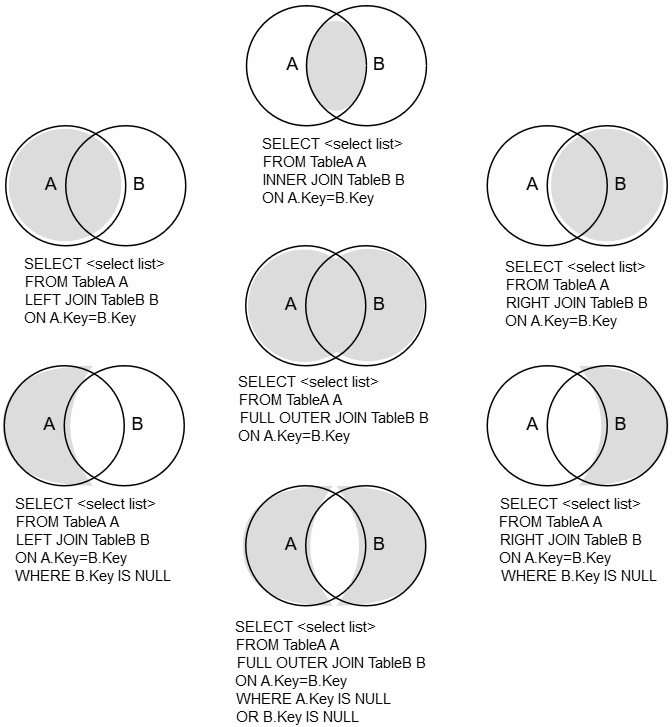
\includegraphics[scale=0.5]{img/sql2.png}
\end{center}
\begin{enumerate}[leftmargin=*]
  \setcounter{enumi}{9}
  \item riscrivi il punto 5.
  \begin{verbatim}
  select I.Nome, Cognome, D.Città
  from Impiegato I join Dipartimento D
       on Dipart = D.Nome
  \end{verbatim}

  \item estrarre tutti gli impiegati che hanno lo stesso cognome (ma diverso nome) di impiegati del dipartimento Produzione
  \begin{verbatim}
  select I1.Nome, I1.Cognome
  from Impiegato I1, Impiegato I2
  where I1.Cognome = I2.Cognome and
        I1.Nome <> I2.Nome and
        I2.Dipart = ‘Produzione’
  \end{verbatim}
  immaginiamo che al momento della definizione degli \hl{alias} (\texttt{I1} e \texttt{I2}) vengano create due diverse tabelle che verranno confrontate tra di loro.
\end{enumerate}

\subsubsection{Order by}
clausola \hl{order by} - ordina in modo ascendente (\hl{asc}) o discendente (\hl{desc})
\begin{enumerate}[leftmargin=*]
  \setcounter{enumi}{11}
  \item estrarre il contenuto della tabella AUTOMOBILE ordinato in base alla marca (in modo discendente) e al modello
  \begin{verbatim}
  select *
  from Automobile
  order by Marca desc, Modello
  \end{verbatim}
\end{enumerate}

\subsubsection{Operatori aggregati}
\hl{count} - torna il numero degli attributi\\
\hl{sum} - torna la somma dei valori dell’espressione\\
\hl{max} - massimo\\
\hl{min} - minimo\\
\hl{avg} - media dei valori
\begin{enumerate}[leftmargin=*]
  \setcounter{enumi}{12}
  \item estrarre il numero di diversi valori dell’attributo Stipendio fra tutte le righe di IMPIEGATO
  \begin{verbatim}
  select count (distinct Stipendio)
  from Impiegato
  \end{verbatim}
\end{enumerate}

\subsubsection{Group by}
clausola \hl{group by} - raggruppa per
\begin{enumerate}[leftmargin=*]
  \setcounter{enumi}{13}
  \item estrarre la somma degli stipendi di tutti gli impiegati dello stesso dipartimento
  \begin{verbatim}
  select Dipart, sum(Stipendio)
  from Impiegato
  group by Dipartimento
  \end{verbatim}
\end{enumerate}

\subsubsection{Predicati su gruppi: having}
predicato \hl{having} - che ha
\begin{enumerate}[leftmargin=*]
  \setcounter{enumi}{14}
  \item estrarre i dipartimenti che spendono più di 100 mila euro in stipendi
  \begin{verbatim}
  select Dipart, sum(Stipendio) as SommaStipendi
  from Impiegato
  group by Dipart
  having sum(Stipendio) > 100
  \end{verbatim}
\end{enumerate}

\subsubsection{Interrogazioni di tipo insiemistico}
\hl{union}\\
\hl{intersect}\\
\hl{except}
\begin{enumerate}[leftmargin=*]
  \setcounter{enumi}{15}
  \item estrarre i nomi e i cognomi degli impiegati
  \begin{verbatim}
  select Nome
  from Impiegato
        union
  select Cognome
  from Impiegato
  \end{verbatim}
\end{enumerate}

\subsubsection{Any}
clausola \hl{any} - la riga soddisfa la condizione se è vero il confronto tra il valore dell’attributo per la riga e almeno uno degli elementi restituiti dall’interrogazione
\begin{enumerate}[leftmargin=*]
  \setcounter{enumi}{16}
  \item estrarre gli impiegati che lavorano in dipartimenti situati a Firenze
  \begin{verbatim}
  select *
  from Impiegato
  where Dipart = any (select Nome
                      from Dipartimento
                      where Città = ‘Firenze’)
  \end{verbatim}
\end{enumerate}

\subsubsection{Sintassi completa}
\begin{verbatim}
SELECT [ DISTINCT ] lista_elementi_selezione
FROM lista_riferimenti_tabella
[ WHERE espressione_condizionale ]
[ GROUP BY lista_colonne ]
[ HAVING espressione_condizionale ]
[ ORDER BY lista_colonne ]
\end{verbatim}



\subsection{Viste}
Mediante l’istruzione \hl{CREATE VIEW} si definisce una vista, ovvero una “tabella virtuale”. Le tuple della vista sono il risultato di una query che viene valutata dinamicamente ogni volta che si fa riferimento alla vista.

\subsubsection{Esempio 1}
\begin{center}
      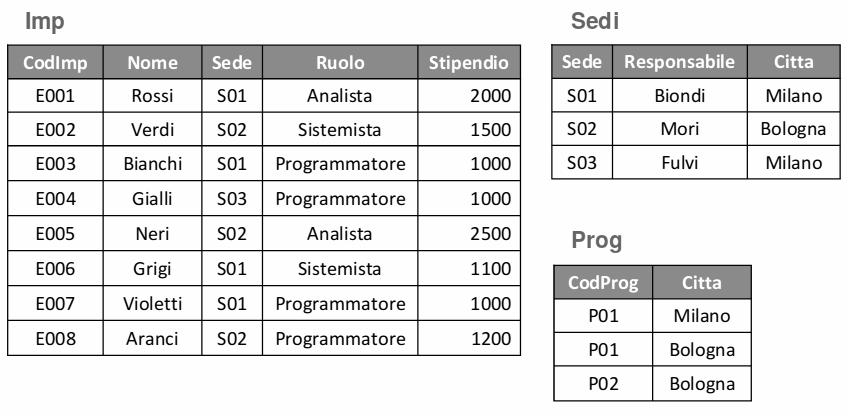
\includegraphics[scale=0.4]{img/sql3.png}
\end{center}
\begin{verbatim}
CREATE VIEW ProgSedi(CodProg, CodSede)
AS  SELECT P.CodProg, S.Sede
    FROM Prog P, Sedi S
    WHERE P.Città=S.Città;

SELECT *
FROM ProgSedi
WHERE CodProg = 'P01'
\end{verbatim}
\begin{center}
      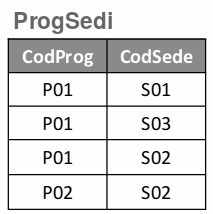
\includegraphics[scale=0.5]{img/sql4.png} \ \ \ \ \ \ \ \ \ \ \ \
      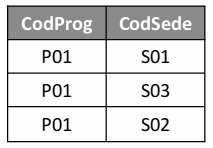
\includegraphics[scale=0.5]{img/sql5.png}
\end{center}

\subsubsection{Esempio 2}
"Trova la sede che ha il massimo numero di impiegati"
\begin{verbatim}
CREATE VIEW NumImp(Sede, NImp)
AS  SELECT Sede, COUNT(*)
    FROM Imp
    GROUP BY Sede;

SELECT Sede
FROM NumImp
WHERE NImp = (SELECT MAX(NImp)
              FROM NumImp)
\end{verbatim}

\subsection{Esercizi}
\subsubsection{Esercizio 1}
ATTORI(\underline{CodAttore}, Nome, AnnoNascita, Nazionalità)\\
RECITA(\underline{CodAttore*, CodFilm*})\\
FILM(\underline{CodFilm}, Titolo, AnnoProduzione, Nazionalità, Regista, Genere)\\
PROIEZIONI(\underline{CodProiezione}, CodFilm*, CodSala*, Incasso, DataProiezione)\\
SALE(\underline{CodSala}, Posti, Nome, Città)
%
\paragraph{Scrivere le interrogazioni SQL che restituiscono le seguenti informazioni}
\begin{enumerate}
\item Il nome di tutte le sale di Pisa
\item Il titolo dei film di F. Fellini prodotti dopo il 1960.
\item Il titolo e il regista dei film di fantascienza giapponesi o francesi prodotti dopo il 1990
\item Il titolo dei film di fantascienza, giapponesi prodotti dopo il 1990 oppure francesi
\item I titolo dei film dello stesso regista di “Casablanca”
\item Il titolo ed  il genere dei film proiettati il giorno di Natale 2004
\item  Il titolo ed  il genere dei film proiettati a Napoli il giorno di Natale 2004
\item  I nomi delle sale di Napoli in cui  il giorno di Natale 2004 è stato proiettato un film con R.Williams
\end{enumerate}

\paragraph{Soluzioni}
\begin{enumerate}
\item
\begin{verbatim}
SELECT Nome FROM Sale
WHERE Città='Pisa'
\end{verbatim}
\item
\begin{verbatim}
SELECT Titolo FROM Film
WHERE Regista='Fellini' AND
      AnnoProduzione>1960
\end{verbatim}
\item
\begin{verbatim}
SELECT Titolo, Regista FROM Film
WHERE Genere='fantascienza' AND
      (Nazionalità='giapponese' OR
      Nazionalità='francese') AND
      AnnoProduzione>1990
\end{verbatim}
\item
\begin{verbatim}
SELECT Titolo FROM Film
WHERE Genere='fantascienza' AND
      ((Nazionalità='giapponese' AND
      AnnoProduzione>1990) OR
      Nazionalità='francese')
\end{verbatim}
\item
\begin{verbatim}
SELECT Titolo FROM Film
WHERE Regista = (SELECT Regista FROM Film
                WHERE Titolo='Casablanca')
\end{verbatim}
\item
\begin{verbatim}
SELECT DISTINCT Titolo, Genere FROM Film
WHERE CodFilm = (SELECT CodFilm FROM Proiezioni
                WHERE DataProiezione='25/12/2004')
\end{verbatim}
\item
\begin{verbatim}
SELECT DISTINCT Titolo, Genere FROM Film
WHERE CodFilm = (SELECT CodFilm FROM Proiezioni
                WHERE DataProiezione='25/12/2004' AND
                CodSala = (SELECT CodSala FROM Sale
                          WHERE Città='Napoli'))
\end{verbatim}
oppure
\begin{verbatim}
SELECT DISTINCT Titolo, Genere FROM Film
JOIN Proiezioni ON Film.CodFilm=Proiezioni.CodFilm
JOIN Sale ON Proiezioni.CodSala=Sale.CodSala
WHERE Città='Napoli' AND
      DataProiezione='25/12/2004'
\end{verbatim}
\item
\begin{verbatim}
SELECT S.Nome FROM Sale S
JOIN Proiezioni P ON S.CodSala=P.CodSala
JOIN Recita R ON P.CodFilm=R.CodFilm
JOIN Attori A ON R.CodAttore=A.CodAttore
WHERE Città='Napoli' AND
      DataProiezione='25/12/2004' AND
      A.Nome='Williams'
\end{verbatim}
oppure
\begin{verbatim}
SELECT Nome FROM Sale S
WHERE CodSala = (SELECT CodSala FROM Proiezioni
                WHERE DataProiezione='25/12/2004' AND
                CodFilm = (SELECT CodFilm FROM Recita
                          WHERE CodAttore = (SELECT CodAttore FROM Attori
                                            WHERE Nome='Williams' )))
\end{verbatim}
\end{enumerate}

\subsubsection{Esercizio 2}
Data la seguente base di dati:\medskip\\
STUDENTE(\underline{mat}, nome, cognome, luogoNascita)\\
ESAME(\underline{mat}, \underline{codCorso}, voto, data)\\
CORSO(\underline{codCorso}, nomeCorso, docente)\medskip\\
Si scrivano le seguenti query SQL:
\begin{enumerate}
  \item Trovare la città in cui sono nati gli studenti che complessivamente hanno superato più esami rispetto agli studenti nati in altre città.
  \begin{verbatim}
    SELECT TOP(1) luogoNascita FROM Studente S
    JOIN Esame E ON S.mat=E.mat
    GROUP BY luogoNascita
    ORDER BY DISC COUNT(mat)
  \end{verbatim}
  \item Trovare nome, cognome e matricola degli studenti che hanno superato l'esame di analisi con voto superiore al voto ottenuto per l'esame di fisica.
  \begin{verbatim}
    SELECT S.nome, S.cognome, S.mat FROM Studente S
    JOIN Esame E1 ON S.mat=E1.mat
    JOIN Esame E2 ON S.mat=E2.mat
    JOIN Corso C1 ON E1.codCorso=C1.codCorso
    JOIN Corso C2 ON E2.codCorso=C2.codCorso
    WHERE C1.nomeCorso='Analisi' AND
          C2.nomeCorso='Fisica' AND
          E1.voto>E2.voto
  \end{verbatim}
  \item Trovare il nome dei corsi di cui studenti omonimi hanno superato l'esame.
  \begin{verbatim}
    SELECT C.nome FROM Corso C
    JOIN ESAME E ON C.codCorso=E.codCorso
    JOIN STUDENTE S1 ON E.mat=S1.mat
    JOIN STUDENTE S2 ON E.mat=S2.mat
    WHERE S1.nome=S2.nome AND
          S1.cognome=S2.cognome AND
          S1.mat<>S2.mat
  \end{verbatim}
\end{enumerate}

\subsubsection{Esercizio 3}
La seguente base di dati descrive l'attività di una società di noleggio di autovetture che ha diverse sedi in alcune città italiane:\medskip\\
SEDE(\underline{nomeSede}, Indirizzo, città, telefono, direttore)\\
AUTOVETTURA(\underline{targa}, modello, annoImmatricolazione, numeroPosti, colore)\\
CLIENTE(\underline{CF}, nome, cognome, telefono, città)\\
CONTRATTO(\underline{auto, cliente, dataNoleggio}, sedeNoleggio, dataConsegna, sedeConsegna)

\begin{enumerate}
  \item Trovare il numero di autovetture noleggiate in ogni città, da clienti con residenza in una città diversa dalla città in cui avviene il noleggio
  \begin{verbatim}
  SELECT C.sedeNoleggio, A.COUNT(targa) FROM Autovettura A
  JOIN Contratto C ON A.targa = C.auto
  JOIN Cliente Cl ON C.cliente = Cl.CF
  WHERE Cl.città<>C.sedeNoleggio
  GROUP BY C.sedeNoleggio
  \end{verbatim}
  \item Trovare i clienti (CF, nome, cognome) che hanno noleggiato almeno due macchine diverse nella stessa sede di noleggio
  \begin{verbatim}
    SELECT DISTINCT C.CF, C.nome, C.cognome, FROM Cliente C
    JOIN Contratto C1 ON C.CF=C1.cliente
    JOIN Contratto C2 ON C.CF=C2.cliente
    JOIN AUTOVETTURA A1 ON C1.auto=A1.targa
    JOIN AUTOVETTURA A2 ON C2.auto=A2.targa
    WHERE C1.sedeNoleggio=C2.sedeNoleggio AND
        A1.targa<>A2.targa
  \end{verbatim}
  \item Trovare la sede di noleggio, indicandone anche la città, che ha realizzato il maggior numero di contratti della durata di un giorno (cioè in cui la macchina sia stata riconsegnata lo stesso giorno in cui è stata noleggiata)
  \begin{verbatim}
    #Raggruppa le righe in base alla sede e alla città
    #e per ogni gruppo effettua il conteggio degli elementi presenti

    CREATE VIEW NoleggiUnGiorno(sede, città, numero)
    AS SELECT S.nomeSede, S.città, COUNT(*)
    FROM Sede S
    JOIN Contratto C ON S.nomeSede=C.sedeNoleggio
    WHERE C.dataNoleggio=C.dataConsegna
    GROUP BY S.nomeSede, S.città;

    SELECT N.sede, N.città
    FROM NoleggiUnGiorno N
    WHERE numero = (SELECT MAX(N1.numero) FROM NoleggiUnGiorno N1)
  \end{verbatim}
\end{enumerate}

\subsubsection{Esercizio 4}
La seguente basi di dati descrive l'archivio di una società di charter che organizza e vende vacanze in barca. La società dispone di una flotta di barche ed organizza viaggi con diverse destinazioni.\medskip\\
VIAGGIO(\underline{idCliente}, \underline{dataPartenza}, \underline{nomeBarca}, Skipper, portoPartenza, portoArrivo, costo)\\
CLIENTE(\underline{idCliente}, nome, cognome, nazione)\\
FLOTTA(\underline{NomeBarca}, modello, lunghezza, posti, annoImmatricolazione)\\
PORTO(\underline{Nome}, nazione, posti, telefono, canaleRadio)
\begin{enumerate}
\item Trovare la nazione che è stata coinvolta nella maggior parte dei viaggi (come porto di arrivo o come porto di partenza, entrambe)
  \begin{verbatim}
  CREATE VIEW Info as SELECT P.nazione, count(*) as Conteggio FROM Porto P
  JOIN Viaggio V1 ON P.nazione = V.portoPartenza
  JOIN Viaggio V2 ON P.nazione = V.portoArrivo
  GROUP BY P.nazione;

  SELECT I.nazione FROM Info I
  WHERE I.Conteggio = SELECT(MAX(I1.Conteggio) FROM Info I1)
  \end{verbatim}
\item Trovare il nome delle barche che non sono mai state affittate
  \begin{verbatim}
  SELECT F.NomeBarca FROM Flotta F
  LEFT JOIN Viaggio V ON F.NomeBarca=V.nomeBarca
  WHERE V.nomeBarca IS NULL
  \end{verbatim}
\item Trovare per ogni porto il costo medio dei viaggi da lì partiti che non abbiamo imbarcato clienti della nazionalità del porto stesso.
  \begin{verbatim}
  SELECT P.Nome, AVG(V.costo)
  FROM Porto P
  JOIN Viaggio V on P.Nome=V.portoPartenza
  JOIN Cliente C on P.nazione<>C.nazione
  GROUP BY P.Nome
  \end{verbatim}
\end{enumerate}

\subsubsection{Esercizio 5}
Data la seguente base di dati:\medskip\\
AGENTE(\underline{matricola}, nome, cognome, telefono, annoNascita, annoIscrizioneAlbo)\\
LOCALE(\underline{idLocale}, tipoLocale, indirizzo, città, mq, codiceProprietario)\\
AFFITTO(\underline{idLocale}, agente, \underline{dataStipulaContratto}, codiceAffittuario, dataFineContratto, costoMensile)\\
VENDITA(\underline{idLocale}, agente, prezzo, \underline{dataVendita}, codiceAcquirente)\\
CLIENTE(\underline{codiceCliente}, nome, cognome, telefono, CF)\medskip
\begin{enumerate}
  \item Trovare codiceCliente, nome, cognome dei clienti che abbiano sia venduto che affittato locali a Milano nel 2010
  \begin{verbatim}
    SELECT C.codiceCliente, C.nome, C.cognome FROM Cliente C
    JOIN Locale L ON C.codiceCliente=L.codiceProprietario
    JOIN Affitto A ON L.idLocale=A.idLocale
    JOIN Vendita V ON L.idLocale=V.idLocale
    WHERE L.città='Milano' AND
          YEAR(A.dataStipulaContratto)='2010' AND
          YEAR(V.dataVendita)='2010'
  \end{verbatim}
  \item Trovare matricola, nome, cognome dell'agente che ha stipulato più contratti di vendita di uffici
  \begin{verbatim}
    #Conteggio è la nuova tabella
    #Contratti è il nome della colonna che contiene count(*)
    #Group by va fatto per forza su tutti gli elementi
    #presenti nel SELECT che non sono generati da un operatore
    #(come count() ad es.)

    CREATE VIEW Conteggio as
    SELECT A.matricola, A.nome, A.cognome, count(*) as Contratti
    FROM Agente A
    JOIN Vendita V ON A.matricola=V.agente
    JOIN Loacle L ON V.idLocale=L.idLocale
    WHERE tipoLocale='ufficio'
    GROUP BY matricola, nome, cognome;

    SELECT C.matricola, C.nome, C.cognome FROM Conteggio C
    WHERE C.Contratti = (SELECT MAX(C1.Contratti) FROM Contratti C1)
  \end{verbatim}
\end{enumerate}
\section{Link utili}
\begin{itemize}[leftmargin=*]
  \item \url{https://www.w3schools.com/sql/}
  \item \url{https://www.html.it/guide/guida-linguaggio-sql/}
  \item \url{http://www.dia.uniroma3.it/~patrigna/didactic/sistemi_informativi/materiale.html}
  \item \url{http://www.di.unito.it/~anselma/lingue/#testi}
  \item \url{http://www.di.unipi.it/~leoni/BDeSI/BD.html}
  \item \url{https://users.dimi.uniud.it/~massimo.franceschet/teatro-sql/}
  \item \url{http://www.star.dist.unige.it/~marco/SI1-SV/materialeDidattico.htm}
  \item \url{http://www.cs.unibo.it/~moretti/teaching.html}
  \item \url{http://www.dii.unisi.it/~franco/Teaching/BasiDiDati/0910/BasiDiDati.php}
  \item \url{http://linuxdidattica.org/docs/fb_db/}
\end{itemize}

\end{document}
